\documentclass[12pt]{article}
\usepackage{preamble}

\pagestyle{fancy}
\fancyhead[LO,LE]{Дополнительные главы \\ высшей математики}
\fancyhead[RO,RE]{Лекции Далевской О. П.}

\fancyfoot[L]{\scriptsize исходники найдутся тут: \\ \url{https://github.com/pelmesh619/itmo_conspects} \Cat}

\renewcommand{\thesection}{}

\begin{document}

    \tableofcontents
    \clearpage

    % begin addchapters1_2024_09_06.tex

    \section{\S 1. Ряды}

    \subsection{1. Числовые ряды. Определения}

    \Mems Числовая последовательность: $\{u_n\} = \{u_1, u_2, \dots, u_n, \dots\}, u_n \in \Real$

    \ExNs{1} Бесконечно убывающая геометрическая прогрессия: $u_n = b q^n, \quad
    \frac{1}{2^n} \stackrel{n = 0,1,\dots}{=} \{1, \frac{1}{2}, \frac{1}{4}, \dots\}$

    \ExNs{2} $u_n = 1, -1, 1, -1, \dots$

    \Def $\{u_n\}$ - последовательность

    $\sum_{n = 1}^{\infty} u_n = u_1 + u_2 + \dots + u_n + \dots$ называется числовым рядом

    \Notas Начальное значение $n$ произвольно (целое)

    \Ex $u_n = \frac{1}{(n - 4)^3}, \quad n = 5, 6, \dots$

    $u_n = \frac{1}{n^3}, \quad n = 2024, 2025, \dots$

    \Notas $u_n$ называется общим членом ряда

    \Nota Существует ли сумма $\sum_{n = 1}^{\infty} u_n$ и в каком смысле?

    \ExN{3} $\sum_{n = 1}^{\infty} n = 1 + 2 + 3 + \dots = \infty$ - существует, но бесконечная

    \ExNs{4} $\sum_{n = 0}^{\infty} (-1)^n = 1 - 1 + 1 - 1 + 1 - 1 + \dots =
    \begin{sqcases}
        0 + 0 + \dots = 0 \\
        1 + 0 + 0 + \dots = 1
    \end{sqcases}$

    \ExNs{5} $\sum_{n = 0}^\infty \frac{1}{2^n} = 1 + \frac{1}{2} + \frac{1}{4} + \dots = 2$

    \Def Частичная сумма ряда $S_n \stackrel{def}{=} \sum_{k = 1}^{n} u_k$

    \Notas Последовательность частичных сумм - $S_1, S_2, S_3, S_4, \dots$

    \Ex $1 + \frac{1}{2} + \frac{1}{4} + \frac{1}{8} + \dots$

    $S_1 = u_1 = 1 \quad S_2 = \frac{3}{2} \quad S_3 = \frac{7}{4} \quad S_4 = \frac{15}{8}$

    $\lim_{n \to \infty} S_n = ?$, но проблема заключается в том, что бы найти формулу для $S_n$

    \Def Если $\exists \lim_{n \to\infty} S_n = S \in \Real$, то ряд $\sum_{n = 1}^\infty u_n$ называют сходящимся,
    а $S$ называют суммой ряда $\sum_{n = 1}^\infty u_n = S$

    \Notas В противном случае ряд расходится, суммы не может быть или она бесконечна

    \Ex Поиск суммы по определению

    $\sum_{n = 1}^\infty \frac{1}{n (n + 1)}$

    $u_n = \frac{1}{n(n + 1)} = \frac{1}{n} - \frac{1}{n + 1}$

    $S_n = \sum_{k = 1}^n u_k = \sum_{k = 1}^n \left(\frac{1}{k} - \frac{1}{k + 1}\right) = 1 - \frac{1}{2} + \frac{1}{2} - \frac{1}{3} + \frac{1}{3} + \dots + \frac{1}{n} - \frac{1}{n + 1} = 1 - \frac{1}{n + 1}$

    $\lim_{n \to \infty} S_n = \lim_{n \to \infty} \left(1 - \frac{1}{n + 1}\right) = 1 = S = \sum_{n = 1}^\infty \frac{1}{n(n + 1)}$

    \Nota При исследовании на сходимость используются эталонные ряды

    \Ex Геометрический ряд (эталонный): \ \ $\sum_{n = 0}^\infty b q^n$

    $S_n = \sum_{k = 0}^n b q^k = b (1 + q + q^2 + q^3 + \dots + q^n) = b \frac{1 - q^n}{1 - q}$

    Исследуем предел $\lim_{n\to\infty} S_n$:

    $|q| < 1 \quad\quad \lim_{n\to\infty} S_n = \frac{b}{1 - q} \lim_{n \to\infty} (1 - q^n) = \frac{b}{1 - q}$

    $|q| > 1 \quad\quad \lim_{n\to\infty} S_n = \infty (q^n \to\infty)$

    $|q| = 1 \quad\quad \lim_{n\to\infty} b \frac{0}{0} ? \quad\quad \sum_{n = 0}^\infty b q^n = \sum_{n = 0}^\infty b = \infty \quad (b \neq 0)$

    $q = -1 \quad\quad \sum_{n = 0}^\infty b (-1)^n$ - расходится (из четвертого примера)

    \Lab Доказать при $q = -1$ по def $(S_n = ?)$\

    \subsection{2. Свойства числовых рядов}

    \Notas Свойства рядов используются в арифметических операциях с рядами и при исследовании на сходимость

    \begin{MyTheorem}
        \ThNs{1} Отбрасывание или добавление конечного числа членов ряда не влияет на сходимость, но влияет на сумму

        $\sum_{n = 1}^\infty u_n$ и $\sum_{n = k > 1}^\infty u_n$ одновременно сходятся или расходятся
    \end{MyTheorem}

    \begin{tcolorbox}
        $\Box$

        $S^u_n = \sum_{n = 1}^{\infty} u_n = u_1 + u_2 + u_3 + \dots + u_k + u_{k + 1} + \dots + u_n + \dots$

        $S^v_n = \sum_{n = k}^\infty v_n \quad\quad u_n = v_n \quad \forall n \geq k$

        $S_n^u = \underset{\sigma \in \Real}{\underbrace{u_1 + u_2 + \dots + u_{k - 1}}} + \underset{S^v_n}{\underbrace{u_{k} + \dots + u_n}} = \sigma + S^v_n$

        $\lim_{n \to \infty} S_n^u = \lim_{n \to \infty} (\sigma + S^v_n) = \sigma + \lim_{n + \infty} S_n^v$

        \smallvspace

        Оба предела либо существуют (либо конечны, либо нет), либо не существуют

        % old proof (basically right but too complicated):

        % $S_n = \sum_{k = 1}^n u_k \quad\quad \sigma_t = \sum_{r = 1}^t v_r \quad\quad v_r = u_{k - 1 + r}$
        %
        % $\lim_{n \to \infty} S_n = \lim_{n \to\infty} (u_1 + u_2 + u_3 + \dots + u_k + u_{k + 1} + \dots + u_n) = u_1 + \dots + u_{k - 1} + \lim_{t \to \infty} \sigma_t$

        $\Box$
    \end{tcolorbox}

    \begin{MyTheorem}
        \ThNs{2} $\sum_{n = 1}^\infty u_n = S \in \Real, \quad \alpha \in \Real$

        Тогда $\alpha \sum_{n = 1}^\infty u_n = \sum_{n = 1}^\infty \alpha u_n = \alpha S$
    \end{MyTheorem}

    \begin{tcolorbox}
        $\Box$ По свойству пределов $\Box$
    \end{tcolorbox}

    \begin{MyTheorem}
        \ThNs{3} $\sum_{n = 1}^\infty u_n = S \in \Real$, $\sum_{n = 1}^\infty v_n = \sigma \in \Real$

        Тогда $\sum_{n = 1}^\infty (u_n \pm v_n) = S \pm \sigma$ - сходится
    \end{MyTheorem}

    \begin{tcolorbox}
        $\Box$ По свойству пределов $\lim_{n \to\infty} (S_n \pm \sigma_n) = \lim_{n \to\infty} S_n \pm \lim_{n \to\infty} \sigma_n = S \pm \sigma$ $\Box$
    \end{tcolorbox}

    \Nota Обратное неверно! Теорема разрешает складывать и вычитать сходящиеся ряды, но из сходимости суммы рядов не следует сходимость каждого из них

    \Exs $\sum_{n = 1}^\infty \frac{1}{n (n + 1)} = 1$, \quad но: $\frac{1}{n (n + 1)} = \frac{1}{n} - \frac{1}{n + 1}$,
    а $\sum_{n = 1}^\infty \frac{1}{n}$ и $\sum_{n = 1}^\infty \frac{1}{n + 1}$ расходятся

    \Nota Докажем расходимость $\sum_{n = 1}^\infty \frac{1}{n}$

    \Exs Гармонический ряд (эталонный)

    $\sum_{n = 1}^\infty u_n = 1 + \frac{1}{2} + \frac{1}{3} + \frac{1}{4} + \frac{1}{5} + \frac{1}{6} + \frac{1}{7} + \frac{1}{8} + \frac{1}{9} + \frac{1}{10} + \frac{1}{11} + \frac{1}{12} + \frac{1}{13} + \frac{1}{14} + \frac{1}{15} + \frac{1}{16} + \dots$

    $\sum_{n = 1}^\infty v_n = 1 + \frac{1}{2} + \frac{1}{4} + \frac{1}{4} + \frac{1}{8} + \frac{1}{8} + \frac{1}{8} + \frac{1}{8} + \frac{1}{16} + \frac{1}{16} + \frac{1}{16} + \frac{1}{16} + \frac{1}{16} + \frac{1}{16} + \frac{1}{16} + \frac{1}{16} + \dots = \\
    \quad = 1 + \frac{1}{2} \cdot 1 + \frac{1}{4} \cdot 2 + \frac{1}{8} \cdot 4 + \frac{1}{16} \cdot 8 + \dots = 1 + \sum_{n = 1}^\infty \frac{1}{2} = \infty$

    А так как нижний ряд почленно меньше верхнего, а нижний расходится, то и верхний расходится

    Так как $u_n \geq v_n$, то $S_n \geq \sigma_n$, тогда $\lim_{n \to\infty} S_n \geq \lim_{n \to\infty} \sigma_n$

    $\sigma_n = 1 + \frac{1}{2} \cdot n \to \infty \Longrightarrow S_n \to \infty$

    \begin{MyTheorem}
        \ThNs{4} Если ряд сходится к числу $S$, то члены ряда можно группировать произвольным образом, не переставляя, и сумма всех рядов будет равна $S$

        Группировка означает выделение различных подпоследовательностей из последовательности частичных сумм
    \end{MyTheorem}

    \begin{tcolorbox}
        $\Box$

        Так как $\lim_{n \to\infty} S_n = S$, то $\lim_{k \to\infty} S_n^{(k)} = S$, где $S_n^{(k)}$ - подпоследовательность $S_n$

        $\Box$
    \end{tcolorbox}

    \Exs Было $\sum (-1)^n = 1 - 1 + 1 - 1 + 1 - 1 + 1 - \dots = \begin{sqcases}
                                                                     0, \\ 1,
    \end{sqcases}$ так как ряд расходится

    \Nota В условиях \Ths важно, что переставлять члены ряда нельзя

    \Exs $\sum_{n = 1}^\infty \frac{(-1)^{n - 1}}{n} = 1 - \frac{1}{2} + \frac{1}{3} - \frac{1}{4} + \frac{1}{5} - \frac{1}{6} + \frac{1}{7} - \frac{1}{8} + \frac{1}{9} - \frac{1}{10} + \frac{1}{11} - \frac{1}{12} + \frac{1}{13} - \frac{1}{14} + \frac{1}{15} + \dots$

    Далее будет доказано, что этот ряд сходится

    Найдем сумму, переставив члены ряда

    $S = \sum_{n = 1}^\infty \frac{(-1)^{n - 1}}{n} = 1 - \frac{1}{2} + \left(\frac{1}{3} - \frac{1}{6}\right) - \frac{1}{4} + \left(\frac{1}{5} - \frac{1}{10}\right) - \frac{1}{8} + \left(\frac{1}{7} - \frac{1}{14}\right) - \frac{1}{12} + \left(\frac{1}{9} - \frac{1}{18}\right) + \dots\\
    S = 1 - \frac{1}{2} \left(1 + \frac{1}{2} - \frac{1}{3} + \frac{1}{4} - \frac{1}{5} + \frac{1}{6}\right) = 1 + \frac{1}{2} \left(-1 - \frac{1}{2} + \frac{1}{3} - \dots\right) =
    1 + \frac{1}{2} \left(-2 + 1 - \frac{1}{2} + \frac{1}{3} + \dots\right) = \frac{1}{2} \left(1 - \frac{1}{2} + \frac{1}{3} - \dots\right) = \frac{1}{2} S$ \ ?!

    \Notas Можно доказать, что в подобных рядах перестановкой членов можно получить любое наперед заданное число

    \Notas Сходящиеся ряды допускают умножение, но непочленное. В действительности используют формулы перемножения рядов (см. литературу)

    $\sum_{n = 1}^\infty u_n = S, \sum_{n = 1}^\infty v_n = \sigma$

    Тогда $\left(\sum_{n = 1}^\infty u_n\right)\left(\sum_{n = 1}^\infty v_n\right) = S\sigma$

    \mediumvspace

    \subsection{3. Условия сходимости рядов}

    \subsubsection{3.1. Необходимое}

    \begin{MyTheorem}
        \Ths $\sum_{n = 1}^\infty u_n = S \in \Real \Longrightarrow \lim_{n \to \infty} u_n = 0$
    \end{MyTheorem}

    \begin{tcolorbox}
        $\Box$

        $\lim_{n \to \infty} S_n = S, \quad \lim_{n\to\infty} (S_n - S_{n - 1}) = 0$

        $\Box$
    \end{tcolorbox}

    \Nota Обратное неверно! (см. гармонический ряд)

    \Ex $\sum_{n = 1}^\infty (2n + 3) \sin \frac{1}{n}$

    $\lim_{n \to \infty} (2n + 3) \sin \frac{1}{n} = \lim_{n \to \infty} (2 + \frac{3}{n}) = 2 \neq 0$

    \subsubsection{3.2. Критерии (Необходимое и Достаточное условия)}

    \Mem Критерий Коши для последовательности: 
    
    $\{x_n\}$ сходится $\Longleftrightarrow \forall \varepsilon > 0 \ \exists \underset{n_0 = n_0 (\varepsilon)}{n_0 \in \Natural} \ | \ \forall m > n > n_0 \ \ |x_m - x_n| < \varepsilon$

    \begin{MyTheorem}
        \Ths (без док-ва) 
        
        $\quad \sum_{n = 1}^\infty u_n$ сходится $\Longleftrightarrow \forall \varepsilon > 0 \ \exists \underset{n_0 = n_0 (\varepsilon)}{n_0 \in \Natural} \ | \ \forall m > n > n_0 \ \ \underset{|S_m - S_n| < \varepsilon}{|u_{n + 1} + \dots + u_m|} < \varepsilon$
    \end{MyTheorem}

    \Nota Хвост ряда попадает в $\varepsilon$-трубу

    \Notas Критерий не удобен для непосредственного исследования на сходимость, в отличии от признаков
% end addchapters1_2024_09_06.tex

% begin addchapters1_2024_09_20.tex

    \subsubsection{3.3. Достаточное условие (признаки сходимости)}

    Здесь мы рассмотрим:

    \begin{enumerate}
        \item Признак сравнения (в неравенствах)
        \item Предельный признак сравнения
        \item Признак Даламбера
        \item Признак Коши (радикальный)
        \item Признак Коши (интегральный)
    \end{enumerate}

    Далее $\sum_{n = 1}^\infty u_n$ - исследуемый ряд, $\sum_{n = 1}^\infty v_n$ - вспомогательный (уже исследован на сходимость),
    для простоты $v_n, u_n > 0$ (для отрицательных доказывается аналогично)

    \mediumvspace

    \begin{MyTheorem}
        \ThNs{1} Признак сравнения (в неравенствах)

        a) $\letsymbol 0 < u_n \leq v_n. \quad$ Тогда $\sum v_n$ сходится $\Longrightarrow \sum u_n$ сходится

        б) $\letsymbol 0 \leq v_n \leq u_n. \quad$ Тогда $\sum v_n$ расходится $\Longrightarrow \sum u_n$ расходится
    \end{MyTheorem}

    \begin{MyProof}
        $\Box$

        а) Строим частичные суммы:

        $\sum v_n$ сходится $\Longleftrightarrow \exists \lim_{n \to \infty} \sigma_n = \sigma \in \Real$

        $S_n, \sigma_n$ возрастают и обе ограничены числом $\sigma$

        Следовательно $\exists \lim_{n \to \infty} S_n = S \leq \sigma$

        Аналогично пункт б)

        $\Box$
    \end{MyProof}

    \begin{MyTheorem}
        \ThNs{2} Предельный признак

        $\lim_{n \to \infty} \frac{u_n}{v_n} = q \in \Real \setminus \{0\} \ \Longrightarrow \
        \begin{sqcases}
            \sum u_n \text{ сходится, если } \sum v_n \text{ сходится} \\
            \sum u_n \text{ расходится, если } \sum v_n \text{ расходится}
        \end{sqcases}$
    \end{MyTheorem}

    \begin{MyProof}
        $\Box$

        По определению предела

        $\exists \lim_{n \to \infty} \frac{u_n}{v_n} = q \in \Real \Longleftrightarrow \forall \varepsilon > 0 \ \exists n_0 \in \Natural \ | \ \forall n > n_0 \ |\frac{u_n}{v_n} - q| < \varepsilon$

        $|\frac{u_n}{v_n} - q| < \varepsilon \Longleftrightarrow q - \varepsilon < \frac{u_n}{v_n} < q + \varepsilon$

        $(q - \varepsilon) v_n < u_n < (q + \varepsilon) v_n$

        а) Если $\sum v_n$ сходится, то из правой части неравенства: $0 < u_n < (q + \varepsilon) v_n$

        По признаку сравнения $\sum u_n$ также сходится

        б) Если $\sum v_n$ расходится, то из левой части неравенства: $0 < (q - \varepsilon) v_n < u_n$

        Тогда по пункту б) \ThNs{1} $\sum u_n$ расходится

        $\Box$
    \end{MyProof}

    \Nota При $q = 0$ можем говорить, что $u_n$ - бесконечно малая высшего порядка, чем $v_n$, а значит, если ряд $v_n$
    сходится, то $u_n$ сходится

    \ExN{1} $\sum_{n = 1}^\infty \frac{1}{n^2} = \sum_{n = 1}^\infty u_n$

    $\sum_{n = 1}^\infty \frac{1}{n(n + 1)} = \sum_{n = 1}^\infty v_n$ сходится

    $\frac{1}{n(n + 1)} = \frac{1}{n^2 + n} > \frac{1}{n^2 + 2n + 1} = \frac{1}{(n + 1)^2}$

    $\sum_{n = 0}^\infty \frac{1}{(n + 1)^2} = \sum_{n = 1}^\infty \frac{1}{n^2}$ сходится по признаку сравнения

    \ExN{2} $\sum_{n = 1}^\infty \frac{1}{n!} = \sum_{n = 1}^\infty u_n$

    $\sum_{n = 1}^\infty \frac{1}{2^n} = \sum_{n = 1}^\infty v_n$ сходится

    Начиная с некоторого $n_0$ $n! > 2^n$. Тогда $u_n < v_n$ при $n > n_0$, по признаку сравнения $\sum_{n = 1}^\infty \frac{1}{n!}$ сходится


    \ExN{3} $\sum_{n = 1}^\infty \arcsin \frac{1}{n}$

    \Nota Члены рядов $u_n$ и $v_n$ - бесконечно малые последовательности. Иначе ряды расходятся по необходимому условию.
    Тогда в \ThNs{2} сравниваются порядки бесконечно малых, и ряды одновременно сходятся или расходятся, если $u_n$ и $v_n$ одного
    порядка малости. По этому принципу подбирается вспомогательный ряд

    $u_n = \arcsin \frac{1}{n} \underset{n \to \infty}{\sim} \frac{1}{n} = v_n \quad\quad \sum_{n = 1}^\infty v_n = \sum_{n = 1}^\infty \frac{1}{n}$ расходится

    \begin{MyTheorem}
        \ThNs{3} Признак Даламбера

        $\sum_{n = 1}^\infty u_n$ - исследуемый, $\exists \mathcal{D} = \lim_{n \to \infty} \frac{u_{n + 1}}{u_n} \in \Real^+$

        \begin{tabular}{ll}
            а) $0 \leq \mathcal{D} < 1$ & $\Longrightarrow \sum u_n$ сходится                                \\

            б) $\mathcal{D} > 1$        & $\Longrightarrow \sum u_n$ расходится                              \\

            в) $\mathcal{D} = 1$        & $\Longrightarrow$ ничего не следует, требуется другое исследование \\
        \end{tabular}
    \end{MyTheorem}

    \begin{MyProof}
        $\Box$

        а) По определению предела $\mathcal{D} = \lim_{n \to \infty} \frac{u_{n + 1}}{u_n}, \ 0 \leq \mathcal{D} < 1 \Longleftrightarrow$

        $\forall \varepsilon > 0 \ \exists n_0 \in \Natural \ | \ \forall n > n_0 \ |\frac{u_{n + 1}}{u_n} - \mathcal{D}| < \varepsilon \quad \Longleftrightarrow \quad \mathcal{D} - \varepsilon < \frac{u_{n + 1}}{u_n} < \mathcal{D} + \varepsilon$

        Так как $0 \leq \mathcal{D} < 1$, можно втиснуть число $r$ между $\mathcal{D}$ и 1: $\mathcal{D} < r < 1$

        Положим $\varepsilon = r - \mathcal{D}$, то есть $\mathcal{D} + \varepsilon = r$

        Смотрим правую часть $\frac{u_{n + 1}}{u_n} < r$ для $\forall n > n_0$, где $n_0 = n_0(\varepsilon), \varepsilon = r - \mathcal{D}$

        $u_{n_0 + 1} < r u_{n_0}$

        $u_{n_0 + 2} < r u_{n_0 + 1} < r^2 u_{n_0}$

        $u_{n_0 + l} < r^l u_{n_0}$

        $\sum_{n = 1}^\infty u_n = \underset{k}{\underbrace{u_1 + u_2 + \dots + u_{n_0 - 1}}} + u_{n_0} + \dots = k + \sum_{m = 1}^\infty v_m $ % u_{n_0} + u_{n_0 + 1} + \dots

        Члены $v_m < r^l u_{n_0}$; $u_{n_0}$ - фикс. число, а $\sum_{l = 1}^\infty r^l$ сходится как геометрический при $|r| < 1$

        Итак ряд $\sum_{l = 1}^\infty r^l u_{n_0}$ сходится и почленно превышает $\sum v_m = \left(\sum u_n\right) - k$

        То есть $\sum u_n$ сходится

        б) \Lab (взять $r$ между $\mathcal{D}$ и $1$, $1 < r < \mathcal{D}$, $\mathcal{D} - r = \varepsilon$)

        Сравнить $\sum u_n$ с $\sum r^l$ (расходящимся)

        $\Box$
    \end{MyProof}

    \ExN{1} $\sum_{n = 1}^\infty \frac{1}{n!} \quad\quad \mathcal{D} = \lim_{n \to \infty} \frac{u_{n + 1}}{u_n} = \lim_{n \to \infty} \frac{n!}{(n + 1)!} = \lim_{n \to \infty} \frac{1}{n + 1} = 0$ - сходится

    \ExN{2} $\sum_{n = 1}^\infty \frac{1}{n} \quad\quad \mathcal{D} = \lim_{n \to \infty} \frac{n}{n + 1} = 1$ - расходится

    $\sum_{n = 1}^\infty \frac{1}{n^2} \quad\quad \mathcal{D} = \lim_{n \to \infty} \frac{n^2}{(n + 1)^2} = 1$ - сходится

    \begin{MyTheorem}
        \ThNs{4} Радикальный признак Коши

        $\sum_{n = 1}^\infty u_n \quad\quad u_n \geq 0$ и $\exists \lim_{n \to \infty} \sqrt[n]{u_n} = K \in \Real$

        а) $0 \leq K < 1 \Longrightarrow \sum u_n$ сходится

        б) $K > 1 \Longrightarrow \sum u_n$ расходится
    \end{MyTheorem}

    \Notas $K = 1$ - ничего не следует

    \begin{MyProof}
        $\Box$

        а) По определению предела $\forall \varepsilon > 0 \ \exists n_0 \in \Natural \ | \ \forall n > n_0 \ |\sqrt[n]{u_n} - K| < \varepsilon$

        $\Longleftrightarrow k - \varepsilon < \sqrt[n]{u_n} < k + \varepsilon$ Положим $\varepsilon = r - K$, где $K < r < 1$

        $\Longrightarrow 0 \leq u_n < r^n$ - геом. ряд с $|r| < 1$, то есть $\sum r^n$ сходится

        б) Аналогично

        $\Box$
    \end{MyProof}

    \ExN{1} $\sum_{n \to \infty} \left(\frac{n}{n + 1}\right)^n \quad\quad K = \lim_{n \to \infty} \left(\frac{n}{n + 1}\right)^n = \lim_{n \to \infty} \frac{n}{n + 1} = 1$

    $\mathcal{D} = \lim_{n \to \infty} \frac{\left(1 - \frac{1}{n + 2}\right)^{n + 1}}{\left(1 - \frac{1}{n + 1}\right)^{n}}$

    Но $\lim_{n \to \infty} u_n = e^{-1} \neq 0$ - необходимое условие не выполняется

    \ExN{2} $\sum_{n = 1}^\infty \left(\frac{n}{n + 1}\right)^{n^2}, \quad\quad K = \lim_{n \to \infty} \sqrt[n]{\left(\frac{n}{n + 1}\right)^n} = e^{-1} < 1$ - сходится

    \begin{MyTheorem}
        \ThNs{5} Интегральный признак Коши

        Если существует $f(x) : [1; +\infty] \to \Real^+, f(x)$ монотонно убывает, $f(n) = u_n$, то $\sum_{n = 1}^\infty u_n$ и $\int_{1}^\infty f(x) dx$ одновременно сходятся или расходятся
    \end{MyTheorem}

    \begin{MyProof}
        $\Box$

        $\int_1^{+\infty} f(x) dx = \lim_{b \to \infty} \int_1^b f(x) dx$

        $\sum_{n = 2}^b u_n = u_2 \cdot 1 + u_3 \cdot 1 + \dots < \int_1^b f(x) dx < u_1 \cdot 1 + u_2 \cdot 1 + \dots = \sum_{n = 1}^{b - 1} u_n$

        Обозначим $\sum_{n = 1}^{b - 1} u_n = S_{b - 1}, \quad \sum_{n = 2}^{b} u_n = S_{b - 1} - u_1 + u_b$

        $0 < S_{b - 1} - u_1 + u_b < \int_1^b f(x) dx < S_{b - 1}$

        $0 < \sum_{n = 1}^{\infty} u_n - u_1 + u_b < \int_1^\infty f(x) dx < \sum_{n = 1}^\infty u_n$

        Если $\int$ сходится, то смотрим левую часть

        Если $\int$ расходится, то смотрим правую часть неравенства

        $\Box$
    \end{MyProof}

    \subsection{4. Знакочередующиеся ряды}

    \Def $\sum_{n = 0}^\infty (-1)^n u_n$ ($u_n > 0$) - знакочередующийся ряд

    \begin{MyTheorem}
        \Ths Признак Лейбница

        Если для знакочередующегося ряда $\sum_{n = 0}^\infty (-1)^n u_n$ верно,
        что \ $\underset{n \to \infty}{u_n \to 0}$ \ и \ $|u_1| > |u_2| > \dots > |u_n|$,
        то ряд $\sum_{n = 0}^\infty (-1)^n u_n$ сходится
    \end{MyTheorem}
% end addchapters1_2024_09_20.tex

% begin addchapters1_2024_10_04.tex

    \begin{MyProof}
        $\Box$

        $\sum_{n = 1}^\infty (-1)^{n + 1} u_n = u_1 - u_2 + u_3 - u_4 + \dots + u_n + \dots$

        $S_{2n} = (u_1 - u_2) + (u_3 - u_4) + \dots + (u_{2n - 1} - u_{2n})$

        Все слагаемые в скобках будут больше нуля, тогда частичные суммы будут возрастать

        $S_{2n} = u_1 - (u_2 - u_3) - (u_4 - u_5) - \dots - (u_{2n - 2} - u_{2n - 1}) - u_{2n} < u_1$

        Здесь же тоже все слагаемые больше нуля - их мы вычитаем из $u_1$ и получаем число гарантированно меньшее $u_1$

        По \Ths о монотонности и ограниченности последовательность $\letsymbol \lim_{n \to \infty} S_{2n} = S \in \Real$

        $S_{2n + 1} = S_{2n} + u_{2n + 1}; \qquad \lim_{n \to \infty} S_{2n + 1} = \lim_{n \to \infty} S_{2n} + \cancelto{0}{\lim_{n \to \infty} u_{2n + 1}} = S \in \Real$

        $\Box$
    \end{MyProof}

    \Exs $\sum_{n = 1}^\infty \frac{(-1)^{n + 1}}{n} = 1 - \frac{1}{2} + \frac{1}{3} - \frac{1}{4} + \dots$

    $u_n = \frac{1}{n} \underset{n \to \infty}{\longrightarrow} 0, \qquad \frac{1}{n} > \frac{1}{n + 1} \Longrightarrow$ ряд сходится

    \Nota Оценка остатка ряда

    Запишем ряд: $\sum_{n = 1}^\infty (-1)^{n + 1} u_n = u_1 - u_2 + u_3 - \dots \pm u_n \mp u_{n + 1} =
    S + \sum_{k = n + 1}^\infty (-1)^{k} u_k = S_n + \underset{\uparrow \text{\LARGE остаток ряда}}{R_n\phantom{ikkkkkkkk}}$

    В доказательстве \Ths было установлено, что сумма ряда не превышает своего первого члена

    \[R_{n + 1} < |(-1)^{k + 1} u_k| = u_k = u_{n + 1}\]

    \Ex $1 - \frac{1}{2} + \frac{1}{4} - \frac{1}{8} + \frac{1}{16} \underset{R_4}{\underbrace{ - \frac{1}{32} + \dots}} = \sum_{n = 0}^\infty (-1)^n \frac{1}{2^n}$

    $|R_4| < \frac{1}{32}$

    Проверка: $-(\frac{1}{32} - \frac{1}{64}) - (\frac{1}{128} - \frac{1}{256}) - \dots = -\sum_{k = 3}^\infty \frac{1}{2^{2k}}$ - \Lab досчитать и сравнить с $\frac{1}{32}$

    \Nota Оценка не работает в знакоположительных рядах

    $1 + \frac{1}{2} + \frac{1}{4} + \frac{1}{8} + \frac{1}{16} + \dots$

    $R_3 = \frac{1}{16} + \frac{1}{32} + \frac{1}{64} + \dots = \frac{1}{16} (1 + \frac{1}{2} + \dots) = \frac{2}{16} = \frac{1}{8} > \frac{1}{16}$

    \Def Знакопеременный ряд

    $\sum_{n = 1}^\infty u_n$, где $u_n$ - любого знака и не все $u_n$ одного знака

    \Ex $1 - \frac{1}{2} + \frac{1}{3} + \frac{1}{4} - \frac{1}{5} - \frac{1}{6} + \frac{1}{7} + \dots$

    \Nota Исследование таких рядов (в том числе знакочередующихся) на сходимость можно проводить при помощи ряда из модулей

    \begin{MyTheorem}
        \Ths Абсолютная сходимость

        $\sum_{n = 1}^\infty |u_n|$ сходится $\Longrightarrow \sum_{n = 1}^\infty u_n$ сходится
    \end{MyTheorem}

    \Mems См. абсолютную сходимость в \href{https://pelmesh619.github.io/itmo_conspects/conspects/calculus/calculus_superconspect.pdf}{несобственных интегралах}

    \begin{MyProof}
        $\Box$

        По критерию Коши:

        $\sum_{n = 1}^\infty |u_n|$ сходится $\Longleftrightarrow$

        $\forall \varepsilon > 0 \ \exists \underset{n_0 = n_0(\varepsilon)}{n_0 \in \Natural} \ | \ \forall m > n > n_0 \quad ||u_n| + |u_{n + 1}| + \dots + |u_m|| < \varepsilon$

        По неравенству треугольника:

        $|u_n| + |u_{n + 1} + \dots + u_m| < |u_n| + |u_{n + 1}| + \dots + |u_m| < \varepsilon$

        $\Box$
    \end{MyProof}

    \Notas Обратное неверно!

    \Ex $\sum_{n = 1}^\infty \frac{(-1)^{n + 1}}{n} = 1 - \frac{1}{2} + \frac{1}{3} + \dots $ сходится

    Но $\sum_{n = 1}^\infty \frac{1}{n}$ расходится

    \Def Если $\sum u_n$ сходится, при том что $\sum |u_n|$ сходится, он называется \textbf{абсолютно сходящимся}

    \Defs Если $\sum u_n$ сходится, при том что $\sum |u_n|$ расходится, он называется \textbf{условно сходящимся}

    \Notas Для абсолютно сходящихся рядов перестановка членов безболезнена и сохраняет сумму ряда

    \Notas На абсолютно сходящиеся ряды распространяются признаки сходимости знакоположительных рядов

    1) Признак сравнения: $|u_n| < |v_n|: \ \sum |v_n|$ сходится $\Longrightarrow \sum |u_n|$ сходится

    2) Предельный признак: $\lim |\frac{u_n}{v_n}| = q \in \Real \setminus \{0\}$

    3) $D = \lim |\frac{u_{n + 1}}{u_n}| < 1$

    4) $K = \lim \sqrt[n]{|{u_n}|} < 1$

    5) $\int_a^\infty f(x)dx$ сравнивается с $\sum |u_n|$

    \clearpage


    \section{\S 2. Функциональные ряды}

    \subsection{1. Определения}

    \Def $\sum_{n = 1}^\infty u_n(x)$, где $u_n(x) : E \subset \Real \to \Real$ называется функциональным

    \Notas При фиксации переменной $x$ ряд становится числовым

    \Exs $\sum_{n = 0}^\infty x^n$

    $x = 2 \quad \sum_{n = 0}^\infty 2^n$ расходится

    $x = \frac{1}{2} \quad \sum_{n = 0}^\infty (\frac{1}{2})^n$ сходится

    Таким образом для $|x| < 1$ ряд будет сходящимся, для $|x| > 1$ расходящимся

    \Def Множество значений $x$, при которых $\sum_{n = 1}^\infty u_n(x)$ сходится, называется областью сходимости

    \Defs Если ряд $\sum_{n = 1}^\infty u_n(x)$ сходится при всех $x$ из некоторого множества $E$, то сумма ряда -
    функция $S(x)$

    \Nota То есть $\exists \lim_{n \to \infty} S_n(x) = S(x)$

    Запишем остаток: $R_n(x) = S(x) - S_n(x)$. Часто удобно исследовать $R_n(x) \to 0$. Также работает критерий Коши

    \begin{MyTheorem}
        \Ths Критерий Коши

        $\sum_{n = 1}^\infty u_n(x)$ сходится в области $D \Longleftrightarrow
        \forall \varepsilon > 0 \ \exists \underset{n_0 = n_0(\varepsilon, x)}{n_0 \in \Natural} \ | \
        \forall m > n > n_0 \ |u_n(x) + u_{n + 1}(x) + \dots + u_m(x)| < \varepsilon$
    \end{MyTheorem}

    \Notas Очень неприятно, что $n_0$ зависит от $\varepsilon$ и всякого $x$

    \Def Равномерная сходимость ряда

    $\sum_{n = 1}^\infty u_n(x)$ равномерно сходится в области $D \overset{def}{\Longleftrightarrow}$

    $\forall \varepsilon > 0 \ \exists \underset{n_0 = n_0(\varepsilon)}{n_0 \in \Natural} \ | \ \forall n > n_0 \ |R_n(x)| < \varepsilon$

    \Nota Доказательства равномерной сходимости по определению сложно, пользуются другими способами

    \begin{MyTheorem}
        \Ths Признак Вейерштрасса

        $\exists \sum_{n = 1}^\infty \alpha_n$ - числовой ряд такой, что $\alpha_n > 0$, $\sum \alpha_n$ сходится,
        $|u_n(x)| \leq \alpha_n \ \forall n$

        Тогда $\sum_{n = 1}^\infty u_n(x)$ равномерно сходящийся

    \end{MyTheorem}

    \Nota Ряд $\sum_{n = 1}^\infty \alpha_n$ называется мажорирующим (то есть преобладающий), 
    а ряд $\sum_{n = 1}^\infty u_n(x)$ - мажорируемым

    \begin{MyProof}
        $\Box$

        $\sum_{n = 1}^\infty \alpha_n$ сходится $\Longleftrightarrow \forall \varepsilon > 0 \ \exists \underset{n_0 = n_0(\varepsilon)}{n_0 \in \Natural} \ | \
        \forall n > n_0 \ |R_n^\alpha| < \varepsilon$

        Заменим на условие $|\alpha_n + \dots + \alpha_m| < \varepsilon$ (кр. Коши)

        $|u_n(x) + \dots + u_m(x)| \leq |u_n(x)| + \dots + |u_m(x)| \leq \alpha_n + \dots + \alpha_m \leq \varepsilon$

        При этом номер $n_0$ зависит только от $\varepsilon$

        $\Box$
    \end{MyProof}

    \Nota Таким образом всякий мажорируемый ряд равномерно сходится, но не всякий равномерно сходящийся ряд мажорируем

    \Nota Установим свойство суммы равномерно сходящегося ряда

    \Exs Рассмотрим ряд $\sum_{n = 1}^\infty (x^{\frac{1}{2n + 1}} - x^{\frac{1}{2n - 1}}) = (x^\frac{1}{3} - x^1) + (x^\frac{1}{5} - x^\frac{1}{3}) + (x^\frac{1}{7} - x^\frac{1}{5}) + \dots;$

    $S_n = x^\frac{1}{2n + 1} - x$

    При $x > 0 \quad \lim_{n \to \infty} S_n = \lim_{n \to \infty} (x^\frac{1}{2n + 1} - x) = 1 - x$

    При $x < 0 \quad \lim_{n \to \infty} S_n = \lim_{n \to \infty} (-\sqrt[2n + 1]{|x|} - x) = -1 - x$

    При $x = 0 \quad S_n = 0$
% end addchapters1_2024_10_04.tex

% begin addchapters1_2024_10_18.tex

    \begin{MyTheorem}
        \Ths Если ряд $\sum_{n = 1}^\infty u_n(x) \ (u_n(x) \in C_{[a, b]})$ мажорируем в $D = [a, b]$, то 
        его сумма $S_x$ непрерывна на $[a, b]$
    \end{MyTheorem}

    \begin{MyProof}
        $\Box$

        $S(x)$ непрерывна на $x \in [a, b] \Longleftrightarrow \Delta S \underset{\Delta x \to 0}{\rightarrow} 0$

        $\Delta S(x) = S(x + \Delta x) - S(x), \ S(x) = S_n(x) + r_n(x)$

        $\Delta S_n(x) = S_n(x + \Delta x) - S_n(x)$

        $\Delta S = S(x + \Delta x) - S(x) = S_n(x + \Delta x) + r_n(x +  \Delta x) - S_n(x) - r_n(x)$

        $\Delta S(x) = \Delta S_n + r_n(x + \Delta x) - r_n(x)$

        $|\Delta S(x)| \leq |\Delta S_n| + |r_n(x + \Delta x)| + |r_n(x)|$

        Ряд $\sum_{n = 1}^\infty u_n(x)$ мажорируем $\Longleftrightarrow \exists$ сходящийся $\sum_{n = 1}^\infty \alpha_n \ \Big| \ |u_n(x) \leq \alpha_n|$
    
        Тогда $\forall \varepsilon > 0 \ \exists N = N(\varepsilon) \ | \ |r_n(x)| < \frac{\varepsilon}{3}$

        и $\forall \varepsilon > 0 \ \exists N = N(\varepsilon) \ | \ |r_n(x + \Delta x)| < \frac{\varepsilon}{3}$ (так как $N$ не зависит от $x$; $x + \Delta x \in [a, b]$) 
    
        $\Delta S_n = S_n(x + \Delta x) - S(x) = u_1(x + \Delta x) - u_1(x) + \dots + u_n(x + \Delta x) - u_n(x)$ - конечная сумма непрерывна

        Сама $S_n(x)$ непрерывна, тогда $\forall \varepsilon > 0 \ $ (при фиксированном $N$) $\exists \delta > 0 \ | \ |\Delta S_n(x)| < \frac{\varepsilon}{3}$ при $|\Delta x| < \delta$

        \bgroup
        \setlength\tabcolsep{1.5pt}
        \begin{tabular}{ccl}
            Итак: $\forall \varepsilon > 0 \ \exists N = N(\varepsilon)$ и $\delta > 0 \ | \ \underset{|\Delta x| < \delta}{\forall x \in D}$ & & $|\Delta S_n(x)| < \frac{\varepsilon}{3}$ \\
            
            & $+$ & $|r_n(x + \Delta x)| < \frac{\varepsilon}{3}$ \\ 
            
            & $+$ & $|r_n(x)| < \frac{\varepsilon}{3}$ \\

            & $=$ & $|\Delta S(x)| < \varepsilon$
        \end{tabular}
        \egroup

        То есть $S(x) \in C_{[a, b]}$

        $\Box$
    \end{MyProof}

    \Nota Не все равномерно сходящиеся мажорируются, но у всех $S(x)$ непрерывна

    Это позволяет определить $\int_{x_0}^y S(x) dx$, а если $S(x) \in C^\prime_{[a, b]}$, то и $\frac{dS(x)}{dx}$

    \begin{MyTheorem}
        \Ths Если ряд мажорируется на $[a, b]$ и $u_n(x)$ непрерывна на $[a, b]$, то определен $\int_{x_0}^y S(x)dx$ и 
        $\int_{x_0}^x S(x)dx  = \sum_{n = 1}^\infty \int_{x_0}^x u_n(x) dx$
    \end{MyTheorem}

    \begin{MyProof}
        $\Box$

        $S(x) = S_n(x) + r_n(x) = u_1(x) + u_2(x) + \dots + u_n(x) + r_n(x)$ - конечное число слагаемых из непрерывных функций
        ($r_n(x)$ как хвост равномерно сходящегося ряда)

        Тогда для $x_0, x \in [a, b] \quad \int_{x_0}^x S(x) = \sum_{k = 1}^n \int_{x_0}^x u_k(x) dx + \int_{x_0}^x r_n(x) dx$ - это будет
        верно, если $\int_{x_0}^x r_n(x) dx \underset{n \to \infty}{\longrightarrow} 0$

        По свойству интегралов $\left|\int_{x_0}^x r_n(x) dx\right| \leq \int_{x_0}^x |r_n(x)| dx$

        $\left|\int_{x_0}^x r_n(x) dx\right| \leq \int_{x_0}^x |r_n(x)| dx < \int_{x_0}^x \varepsilon_n dx = \underset{\varepsilon_n \to 0}{\varepsilon_n (x - x_0)}$ ($x, x_0$ - фикс.)

        То есть $\lim_{n \to \infty} \int_{x_0}^x r_n(x) dx = 0$

        $\lim_{n \to \infty} \int_{x_0}^x S(x) dx = \lim_{n \to \infty} \sum_{k = 1}^n \int_{x_0}^x u_k(x) dx + \lim_{n \to \infty} \int_{x_0}^x r_n(x) dx$

        $\int_{x_0}^x S(x) dx = \sum_{n = 1}^\infty \int_{x_0}^x u_n(x) dx$

        $\Box$
    \end{MyProof}

    \Nota Почленно интегрируются не просто равномерно сходящиеся, а мажорируемые, иначе остаток необязательно стремится к 0

    \begin{MyTheorem}
        \Ths $\sum_{n = 1}^\infty u_n(x)$ мажорируем на $[a, b]$ и $u_n(x) \in C^\prime_{[a, b]}$

        Тогда $S^\prime(x) = \sum_{n = 1}^\infty u^\prime_n(x)$
    \end{MyTheorem}

    
    \begin{MyProof}
        $\Box$

        Пусть $g(x) = \sum_{n = 1}^\infty u^\prime_n(x)$. Докажем, что $g(x) = S^\prime(x)$

        $\int_{x_0}^x g(x)dx = \int_{x_0}^x \left(\sum_{n = 1}^\infty u^\prime_n(x)\right) dx = \sum_{n = 1}^\infty 
        \left(\int_{x_0}^x u_n^\prime (x)dx\right) = u_1(x) \Big|_{x_0}^x + u_2(x) \Big|_{x_0}^x + \dots$

        $ = (u_1(x) - u_1(x_0)) + (u_2(x) - u_2(x_0)) + \dots = S(x) - S(x_0)$ - разность сходящихся рядов

        $\int_{x_0}^x g(x) dx = S(x) - S(x_0) \Longrightarrow \left(\int_{x_0}^x g(x) dx\right)^\prime = g(x) = S^\prime(x)$

        $\Box$
    \end{MyProof}

    \subsection{2. Степенные ряды}

    \Def $\sum_{n = 0}^\infty c_n(x - x_0)^n, \ c_n \in \Real, x_0 \in \Real$ - степенной ряд с центром $x_0$ (в точке $x_0$, по степеням $(x - x_0)$)

    \Nota В частности $\sum_{n = 1}^\infty c_n x^n$ - степенной с центром в $x_0 = 0$

    $\sum_{n = 0}^\infty c_n(x - x_0)^n$ легко сводится заменой $x - x_0 = t$ к $\sum_{n = 0}^\infty c_n t^n$

    \begin{MyTheorem}
        \ThNs{Абеля} 

        1) $\sum_{n = 0}^\infty c_n x^n$ сходится в точке $x_1$. Тогда ряд сходится для любого $x$, который $|x| < |x_1|$

        2) $\sum_{n = 0}^\infty c_n x^n$ расходится в точке $x_2$. Тогда ряд расходится $\forall x \ |x| > |x_2|$
    \end{MyTheorem}

    \begin{MyProof}
        $\Box$

        1) В точке $x_1$ $\sum_{n = 0}^\infty c_n x_1^n = c_0 + c_1 x_1 + c_2 x_1^2 + \dots$ - числовой ряд, сходящийся

        В точке $x \ (|x| < |x_1|) \quad \sum_{n = 0}^\infty c_n x^n = c_0 + c_1 x + c_2 x^2 + \dots = 
        c_0 + c_1 x_1 \frac{x}{x_1} + c_1 x_1^2 \frac{x^2}{x_1^2} + \dots$ 

        Для этого ряда докажем абсолютную сходимость

        $\sum_{n = 0}^\infty |c_n x^n| = |c_0| + |c_1 x_1| \left|\frac{x}{x_1}\right| + |c_1 x_1^2| \left|\frac{x^2}{x_1^2}\right| + \dots$

        При этом ряд $\sum_{n = 0}^\infty c_n x_1^n$ сходится $\Longrightarrow \exists M > 0 \ : \ |c_n x_1^n| \leq M$

        И $\left|\frac{x^k}{x_1^k}\right| < 1$, так как $|x| < |x_1|$

        Тогда $|c_0| + |c_1 x_1| \left|\frac{x}{x_1}\right| + |c_1 x_1^2| \left|\frac{x^2}{x_1^2}\right| + \dots + |c_k x_1^k| \left|\frac{x^k}{x_1^k}\right| < 
        M\left(1 + \left|\frac{x}{x_1}\right| + \left|\frac{x}{x_1}\right|^2 + \dots + \left|\frac{x}{x_1}\right|^k\right)$ - геометрическая прогрессия с $|q| < 1$

        Таким образом $\sum_{n = 0}^\infty |c_n x^n| \sim M\sum_{n = 0}^\infty \left|\frac{x}{x_1}\right|^n$, который сходится

        Ряд $\sum_{n = 0}^\infty c_n x^n$ абсолютно сходится (и равномерно?)

        б) От противного, используя пункт а)

        $\Box$
    \end{MyProof}

    \smallvspace

    \begin{minipage}{\textwidth}
        \begin{wrapfigure}{r}{0pt}
            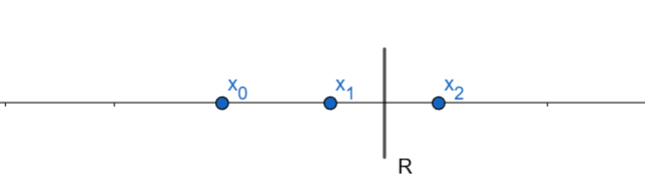
\includegraphics[width=0.4\textwidth]{addchapters1/images/addchapters1_2024_10_18_1}
        \end{wrapfigure}

        \Nota Заметим, что должно существовать такое $R$, для которого для всех $x$ меньше $R$ ряд сходится

        Зафиксируем между $x_0$ и $R$ число $x_0 < r < R$ - тогда $\sum c_n r^n$ - мажорирует $c_n x^n$, то есть ряд сходится равномерно

        \Def $R \in \Real^+ \ \Big| \ \forall |x| < R $ ряд сходится, а $\forall |x| > R$ ряд расходится, тогда $R$ называют радиусом сходимости
        
        \begin{wrapfigure}{r}{0pt}
            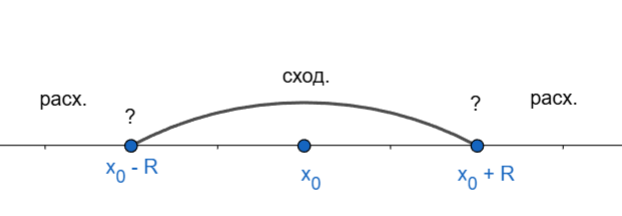
\includegraphics[width=0.4\textwidth]{addchapters1/images/addchapters1_2024_10_18_2}
        \end{wrapfigure}

        Для сдвинутого ряда $\sum_{n = 0}^\infty c_n (x - x_0)^n \quad \forall x: \ |x - x_0| < R$ - сходится; $\forall x: \ |x - x_0| > R$ - расходится
        
        Сходимость ряда в $x_0 \pm R$ нужно проверять специально

        \Nota Чаще всего исследование на сходимость проводится по признакам Даламбера, Коши

        \Ex $\sum_{n = 1}^\infty \frac{x^n}{n} (-1)^{n + 1}$

    \end{minipage}


    $\lim_{n \to \infty} \left|\frac{u_{n+1}}{u_n}\right| = \lim_{n \to \infty} \frac{1}{n + 1} |x|^{n + 1} \frac{n}{|x|^n} = \lim_{n \to \infty} |x| = |x| < 1$

    Предварительно $D = (-1; 1)$. 
    
    Далее, рассмотрим $x = \pm 1$: 
    
    $\quad (x = 1): \sum_{n = 1}^\infty \frac{(-1)^{n + 1}}{n}$ - сходится

    $\quad (x = -1): \sum_{n = 1}^\infty \frac{-1}{n}$ - расходится

    Итак, $D = (-1; 1]$

    \subsection{3. Ряд Тейлора}

    \Mem Формула Тейлора: $f(x) \in C^{n + 1}_{U_\delta (x_0)}$, тогда $f(x) \overset{x \in U_\delta (x_0)}{=\joinrel=\joinrel=} f(x_0) + 
    \frac{f^\prime (x_0)}{1!} (x - x_0) + \frac{f^{\prime\prime} (x_0)}{2!} (x - x_0)^2 + \dots + \frac{f^{(n)} (x_0)}{n!} (x - x_0)^n + \frac{f^{(n + 1)} (\xi)}{(n + 1)!} (x - x_0)^{n + 1}$

    Чтобы $f(x)$ в пределе равнялось $\sum_{n = 0}^\infty \frac{f^{(n)}(x_0)}{n!} (x - x_0)^n$, нужно, чтобы $r_n(x) \to 0$
% end addchapters1_2024_10_18.tex

% begin addchapters1_2024_11_01.tex

    Формула: $f(x) \in C^\infty_{U_0(x_0)}$ и $R_n(x) = \frac{f^{(n + 1)}(\xi)}{(n + 1)!} (x - x_0)^{n + 1}$, $\xi$ между $x$ и $x_0$

    \begin{MyTheorem}
        \Ths Если $R_n(x) \underset{n \to \infty}{\longrightarrow} 0$, то $f(x) = \sum_{n = 0}^\infty \frac{f^{(n)}(x_0)}{n!} (x - x_0)^n$ - ряд Тейлора
    \end{MyTheorem}

    \Nota Если $x_0 = 0$, то ряд Маклорена 

    \smallvspace

    \subsubsection{3.1. Стандартные разложения элементарных функций}

    \smallvspace

    1$^\circ$ $e^x = \sum_{n = 0}^\infty \frac{x^n}{n!} = 1 + x + \frac{x^2}{2} + \frac{x^3}{6} + \dots$

    \Notas $e^x - 1 = x + \frac{x^2}{2} + \dots \qquad e^x - 1 \underset{x \to 0}{\sim} x$

    \mediumvspace

    2$^\circ$ $\sin x = \sum_{n = 0}^\infty \frac{(-1)^n}{(2n + 1)!}x^{2n + 1} = x - \frac{x^3}{3!} + \frac{x^5}{5!} + \dots$

    \Notas $\sin x \underset{x \to 0}{\sim} x$

    \mediumvspace

    3$^\circ$ $\cos x = \sum_{n = 0}^\infty \frac{(-1)^n}{(2n)!}x^{2n} = 1 - \frac{x^2}{2!} + \frac{x^4}{4!} + \dots$

    \Notas $1 - \cos x \underset{x \to 0}{\sim} \frac{x^2}{2}$

    \mediumvspace

    4$^\circ$ $\mathrm{sh} x, \mathrm{ch} x$ \hfill \Defs $\mathrm{sh} x = \frac{e^x - e^{-x}}{2}, \mathrm{ch} x = \frac{e^x + e^{-x}}{2}$
    
    Сложим и вычтем ряды для $e^x$ и $e^{-x}$

    Причем $e^{-x} \underset{x, t \in u(0)}{\overset{t = -x}{=\joinrel=\joinrel=}} e^t = \sum_{n = 0}^\infty \frac{t^n}{n!} = \sum_{n = 0}^\infty \frac{(-1)^n x^n}{n!} = 1 - x + \frac{x^2}{2!} - \frac{x^3}{3!} + \dots$

    Из этого получаем:

    $\mathrm{sh} x = x + \frac{x^3}{3!} + \frac{x^5}{5!} + \dots = \sum_{n = 0}^\infty \frac{x^{(2n + 1)}}{(2n + 1)!}$

    $\mathrm{ch} x = 1 + \frac{x^2}{2!} + \frac{x^4}{4!} + \dots = \sum_{n = 0}^\infty \frac{x^{(2n)}}{(2n)!}$

    \underline{Формула Эйлера}

    $e^{ix} = \sum_{n = 0}^\infty \frac{(ix)^n}{n!} = 1 + ix - \frac{x^2}{2!} - \frac{ix^3}{3!} + \dots = (1 - \frac{x^2}{2!} + \dots) + i(x - \frac{x^3}{3!} + \dots) = \cos x + i\sin x$

    \fbox{$e^{ix} = \cos x + i\sin x$}

    \mediumvspace

    5$^\circ$ Биномиальный ряд

    $f(x) = (1 + x)^m, n \in \mathrm{Q}$

    Заметим, что $f^\prime(x) = m(1 + x)^{m - 1}$

    $(1 + x)f^\prime(x) = m (1 + x)^m = m f(x)$

    Получаем дифференциальное уравнение: $(1 + x)f^\prime(x) = mf(x)$

    \Notas Если дополнить ДУ начальными условиями, то задача Коши будет решаться единственным образом, 
    то есть, найдя ряд $S(x) = \sum_{k = 0}^{\infty} a_k x^k$ как единственное решение,
    получим, что $S(x) = f(x)$ и не надо исследовать остаток $R_n$ на убывание к нулю

    Задача Коши:

    \begin{cases}
        (1 + x) f^\prime(x) = m f(x) \\
        f(0) = 1
    \end{cases}

    Будем искать решение в виде ряда $S(x) = a_0 + a_1 x + a_2 x^2 + \dots + a_k x^k + \dots$

    $S^\prime(x) = a_1 + 2a_2 x + 3a_3 x^2 + \dots + k a_k x^{k - 1} + \dots$

    $(1 + x) S^\prime(x) = a_1 + (a_1 + 2a_2)x + (2a_2 + 3a_3) x^3 + \dots + (k a_k + (k + 1) a_{k + 1})x^k + \dots$

    $mS(x) = ma_0 + ma_1 x + ma_2 x^2 + \dots + m a_k x^k + \dots$

    Начальные условия: $a_0 = 1$. Тогда приравниваем коэффициенты: $a_1 = m, a_2 = \frac{m(m - 1)}{2}, a_3 = \frac{m(m - 1)(m - 2)}{2 \cdot 3}$

    Выявили закономерность: $a_k = \frac{m(m - 1)(m - 2)\dots(m - k + 1)}{k!}$

    Таким образом: $(1 + x)^m = \sum_{k = 0}^\infty C_m^k x^k$

    При $m \in \Natural$ ряд - конечная сумма, при остальных - бесконечная

    \Lab $\frac{1}{\sqrt{1 - x^2}} = (1 + (-x^2))^{-\frac{1}{2}} = (\mathrm{arcsin} x)^\prime \qquad \int_0^t \frac{dx}{\sqrt{1 - x^2}} = \mathrm{arcsin} t$

    \mediumvspace

    6$^\circ$ $\ln(1 + x)$

    $(\ln(1 + x))^\prime = \frac{1}{1 + x} = \frac{1}{1 - (-x)} = \frac{1}{1 - x} = \sum_{n = 0}^\infty t^n = 
    \sum_{n = 0}^\infty (-1)^n x^n$

    $\ln(1 + x) = \int_0^x (\sum_{n = 0}^\infty (-1)^n y^n) dy = \sum_{n = 0}^\infty (-1)^n \int_0^x y^n dy = 
    \sum_{n = 0}^\infty (-1)^n \frac{x^{n + 1}}{n + 1} = x - \frac{x^2}{2} + \frac{x^3}{3} - \frac{x^4}{4} + \dots$
    
    Интервал сходимости: $\lim_{n \to \infty} \left|\frac{u_{n + 1}}{u_n}\right| = 
    \lim_{n \to \infty} \left|\frac{x^{n + 1} n}{(n + 1) x^n}\right| = |x| < 1 \quad D = (-1, 1)$

    При $x = 1 \quad \ln(1 + x) = 1 - \frac{1}{2} + \frac{1}{3} - \frac{1}{4} + \dots$ - сходится $\quad D = (-1, 1]$

    \Notas Сходимость остатка требует исследования

    \Nota Заметим, если $x = \frac{1}{k}$, где $k \in \Natural$, то $\ln(1 + \frac{1}{k}) = \ln\frac{k + 1}{k} = \ln (k + 1) - \ln k$ - рекуррентная формула
    логарифмов натуральных чисел

    \mediumvspace

    7$^\circ$ $\mathrm{arctg} x$ - \Lab ($(\mathrm{arctg} x)^\prime = \frac{1}{1 + x^2}$)

    \subsubsection{3.2. Приложения}

    \ExNs{1} $I = \int_0^{\frac{1}{2}} \frac{\sin x}{x} dx \hfill x = \frac{1}{2} \in u(0)$

    $\frac{\sin x}{x} = 1 - \frac{x^2}{3!} + \frac{x^4}{5!} - \dots$

    $I = \int_0^{\frac{1}{2}} (1 - \frac{x^2}{3!} + \frac{x^4}{5!} - \dots) dx = x - \frac{x^3}{3 \cdot 3!} + \frac{x^5}{5 \cdot 5!} + \dots \Big|_{0}^{\frac{1}{2}} = 
    \frac{1}{2} - \frac{1}{8 \cdot 3 \cdot 6} + \frac{1}{32 \cdot 5 \cdot 120} - \cdot$

    Ряд знакопеременный - можем найти такой $u_n$, который будет меньше заданной точности вычисления $\varepsilon$

    \ExN{2} $\int_0^{a} e^{-x^2} dx = \int_0^a (1 + (-x^2) + \frac{x^4}{2!} + \dots) dx = x - \frac{x^3}{2} + \frac{x^5}{10} + \dots \Big|_0^a = a - \frac{a^3}{5} + \frac{a^5}{10} - \dots$

    Отсюда были вычислены таблицы для функции Лапласа $\Phi(a) = \frac{1}{\sqrt{2\pi}} \int_0^a e^{-\frac{x^2}{2}} dx$

    \ExN{3} Вычисление пределов

    $\lim_{x \to 0} \frac{\sin x - \mathrm{arctg} x}{x^3} = \lim_{x \to 0} \frac{(x - \frac{x^3}{3!} + \frac{x^5}{5!} + \dots) - (x - \frac{x^3}{3} + \frac{x^5}{5} - \frac{x^7}{7} + \dots)}{x^3} = 
    \lim_{x \to 0} \frac{-x^3 (\frac{1}{3!} - \frac{1}{3}) + o(x^3)}{x^3} = \frac{1}{6}$

    \subsection{4. Ряды Фурье}

    \Mem Линейное функциональное пространство со скалярным произведением

    $f(x) \in C_{[a,b]}$

    Скалярное произведение $(f, g) = \int_a^b f(x)g(x) dx$

    Из этого норма $\|f\| = \sqrt{(f,f)} = \left(\int_a^b f^2(x) dx\right)^\frac{1}{2}$

    Главное приложение евклидовых пространств - задача о перпендикуляре: найти перпендикуляр $h$ из конца вектора $f$ на подпространство $L^\prime$.
    Иначе: ищем расстояние $\|f - h\|$ (метрика) или ортогональную проекция $f_0$ вектора $f$ на $L^\prime$, такую, что $f_0 + h = f$

    Будем искать $f_0$, задав подпространство $L^\prime$ множеством функций $\{\sin mx, \cos mx\}$

    Тригонометрические функции полезны для описания периодических явлений

    Раньше рассматривали тригонометрический многочлен

    $T_m(x) = \frac{a_0}{2} + b_1 \sin x + a_1 \cos x + \dots + b_m \sin mx + a_m \cos mx$

    Дальше стоит задача: при каких $a_i, b_i$ многочлен $T_m(x)$ будет наименее отстоящим от данной $f(x)$

    % задача о трех перпендикулярах
% end addchapters1_2024_11_01.tex

% begin addchapters1_2024_11_15.tex

    \Mem Решаем задачу о перпендикуляре, ищем $f_0$ - наименьшую из проекций и минимально отстоящую от $f$

    Координаты $f_0$ в выбранном ортонормированном базисе $L^\prime$ равны соответствующим координатам $f$ в этом базисе

    $f_0 = \underset{k = \dim L^\prime, n = \dim L}{f_1 e_1 + f_2 e_2 + \dots + f_k e_k} = 
    (f, e_1) e_1 + (f, e_2) e_2 + \dots + (f, e_k) e_k$

    $(f, e_1) = \int_a^b f(x) e_1(x) dx$

    \Nota Итак, $\letsymbol L \in C_{[-\pi, \pi]}, L^\prime = l_{\{1, \sin x, \cos x, \sin 2x, \cos 2x, \dots\}}$

    Тогда можно искать многочлен $P_n(x) = \frac{a_0}{2} + a_1 \cos x + b_1 \sin x + \dots + a_n \cos nx + b_n \sin x$, который
    наилучшим образом приближает $f(x)$

    Если нормировать систему $\{\sin nx, \cos nx\}$, то коэффициентами многочлена $P_n(x)$ будут скалярные произведения
    $f(x)$ на функция ортонормированной системы. 
    
    Получим $\left\{\frac{1}{2\pi}, \frac{\sin x}{\pi}, \frac{\cos x}{\pi}, \dots, \frac{\sin nx}{\pi}, \frac{\cos nx}{\pi}\right\}$

    {
        \begin{tabular}{l|l|l}
            \cline{2-2}
            Тогда, & $\frac{a_0}{2} = \frac{1}{2\pi} \int_{-\pi}^\pi f(x) dx$ & \\
            & $a_k = \frac{1}{\pi} \int_{-\pi}^\pi f(x) \cos kx dx$ & - коэффициенты Фурье \\
            & $b_k = \frac{1}{\pi} \int_{-\pi}^\pi f(x) \sin kx dx$ & \\
            \cline{2-2}
        \end{tabular}
    }

    \Nota Если увеличивать степень $n$, то получим ряд Фурье. Запишем формально:

    $\frac{a_0}{2} + \sum_{n = 1}^\infty (a_n \cos nx + b_n \sin nx)$ - сходится ли этот ряд и сходится ли к $f(x)$?

    Ответ дает теорема (доказательство будет приведено позже)

    \begin{MyTheorem}
        \Ths $f(x)$ - $2\pi$-периодична, на $[-\pi, \pi]$ $f(x)$ - кусочно монотонна и ограничена (то есть имеет конечное число конечных разрывов). 
        Тогда в точках непрерывности $f(x)$ представляется рядом Фурье:
        
        \[f(x) = \frac{a_0}{2} + \sum_{n = 1}^\infty (a_n \cos nx + b_n \sin nx) = S(x)\]

        а в точках разрыва $S(x_0) = \frac{1}{2} (f(x_0 + 0) + f(x_0 - 0))$
    \end{MyTheorem}

    Сейчас только тригонометрический ряд Фурье, хотя подобное разложение возможно 
    по различным ортогональным системам функций

    \Nota В концах отрезках $[-\pi, \pi]$ $f(x)$ может быть не определена, но в любом случае ограничена $S(\pi) = S(-\pi) = \frac{1}{2} (f(-\pi + 0) + f(\pi - 0))$

    \mediumvspace

    \underline{Разложение периодичных функций} (на $[-\pi, \pi]$)

    1$^\circ$: $f(x) = x$ на $[-\pi, \pi]$, $f(x + 2\pi) = f(x)$

    $\frac{a_0}{2} = \frac{1}{2\pi} \int_{-\pi}^\pi x dx = 0$

    $a_n = \frac{1}{\pi} \int_{-\pi}^\pi x \cos nx dx = 0$

    $b_n = \frac{1}{\pi} \int_{-\pi}^\pi x \sin nx dx = \frac{-2}{\pi n} \int_{0}^\pi xd\cos nx = -\frac{2}{\pi n} \left(x \cos nx \Big|_0^\pi - \cancelto{0}{\int_0^\pi \cos nx dx}\right) = 
    -\frac{2}{\pi n} x \cos nx \Big|_0^\pi = -\frac{2}{n} \cos \pi n = \begin{sqcases}\frac{-2}{n}, & n = 2m \\ \frac{2}{n}, & n = 2m + 1\end{sqcases} = \frac{2}{n} (-1)^{n + 1}$

    Итак $f(x) = \sum_{n = 1}^\infty \frac{(-1)^{n + 1} \cdot 2}{n} \sin nx$

    \begin{center}
        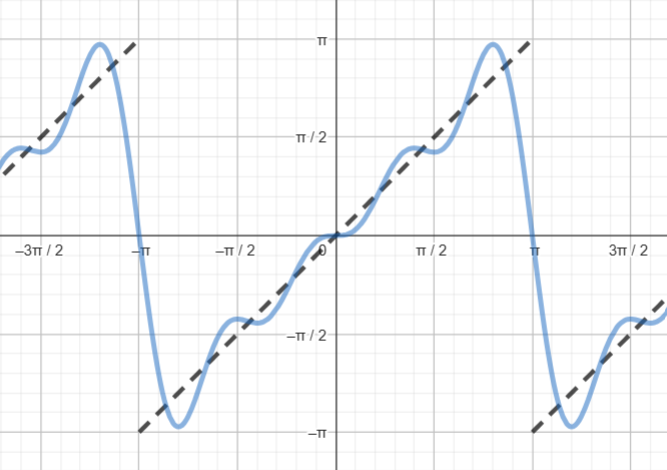
\includegraphics[width=0.5\textwidth]{addchapters1/images/addchapters1_2024_11_15_1}
    \end{center}

    2$^\circ$: $f(x) = \begin{cases}1 & \text{на } [0, \pi] \\ -1 & \text{на } [-\pi, 0)\end{cases}$ на $[-\pi, \pi]$

    $\frac{a_0}{2} = \frac{1}{2\pi} \int_{-\pi}^\pi f(x) dx = 0$

    $a_n = \frac{1}{\pi} \int_{-\pi}^\pi f(x) \cos nx dx = 0$

    $b_n = \frac{1}{\pi} \int_{-\pi}^\pi f(x) \sin nx dx = \frac{1}{\pi} \left(-\int_{-\pi}^0 \sin nx dx + \int_0^\pi \sin nx dx\right) = 
    \frac{1}{2n} \left(\int_{-\pi}^0 d\cos nx - \int_0^\pi d\cos nx\right) = \frac{1}{\pi n} \left(\cos nx \Big|_{-\pi}^0 - \cos nx \Big|_0^\pi\right) = 
    \frac{1}{\pi n} (1 - \cos \pi n - \cos \pi n + 1) = \frac{2}{\pi n}(1 - \cos \pi n) = \frac{4}{\pi (2m - 1)}$

    $f(x) = \sum_{m = 1}^\infty \frac{4}{\pi (2m - 1)} \sin (2m - 1) x$

    \begin{center}
        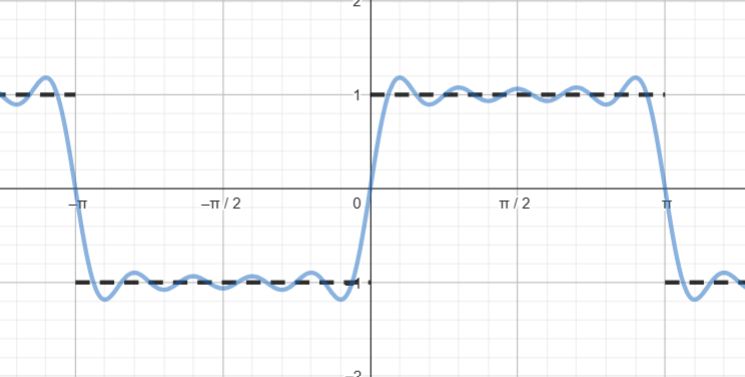
\includegraphics[width=0.5\textwidth]{addchapters1/images/addchapters1_2024_11_15_2}
    \end{center}

    \Nota Заметим, что если $f(x)$ - четная, то $b_n = 0$, а если нечетная, то $a_n = 0$. Иногда в задаче
    требуется разложить $f(x)$, заданную только на отрезке $[0, \pi]$. Такую функцию можно продолжить четным
    или нечетным образом на $[-\pi, \pi]$. Говорят о разложении в ряд по косинусам и синусам соответственно

    3$^\circ$: $f(x) = \pi - x, \quad x \in [0, \pi]$

    Дополним $f(x)$ двумя способами

    \begin{multicols}{2}
        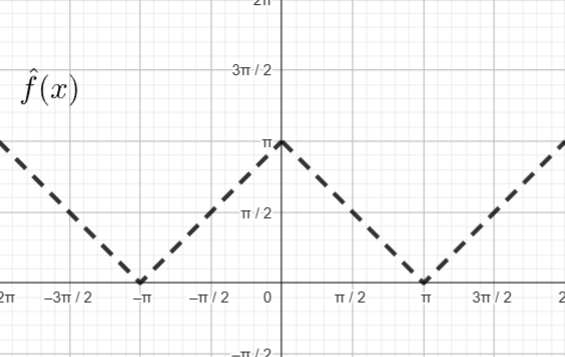
\includegraphics[width=0.5\textwidth]{addchapters1/images/addchapters1_2024_11_15_4}

        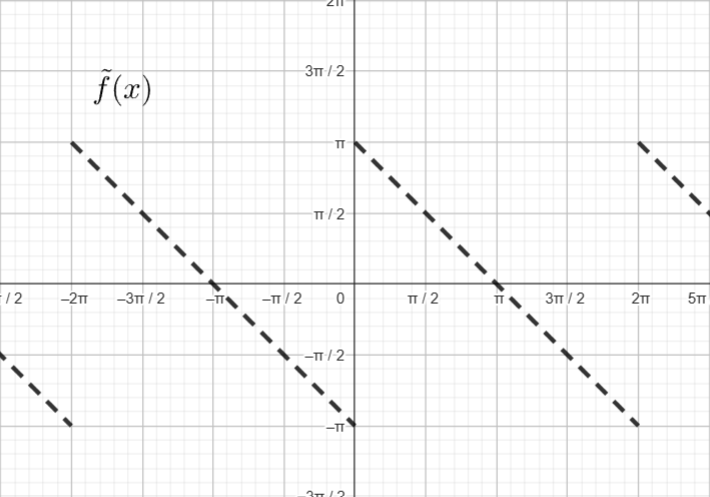
\includegraphics[width=0.5\textwidth]{addchapters1/images/addchapters1_2024_11_15_3}
    \end{multicols}

    В ряд Фурье раскладывются периодические функции $\hat{f}, \tilde{f}$

    \Lab $\hat{f}(x) = \frac{a_0}{2} + \sum_{n = 1}^\infty a_n \cos nx \quad\quad\quad \tilde{f}(x) = \sum_{n = 1}^\infty b_n \sin nx$

    \mediumvspace

    \begin{multicols}{2}
        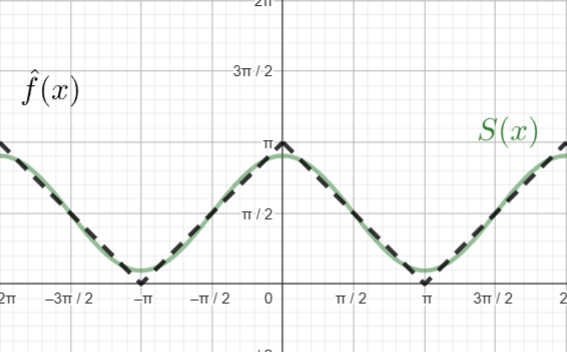
\includegraphics[width=0.5\textwidth]{addchapters1/images/addchapters1_2024_11_15_5}

        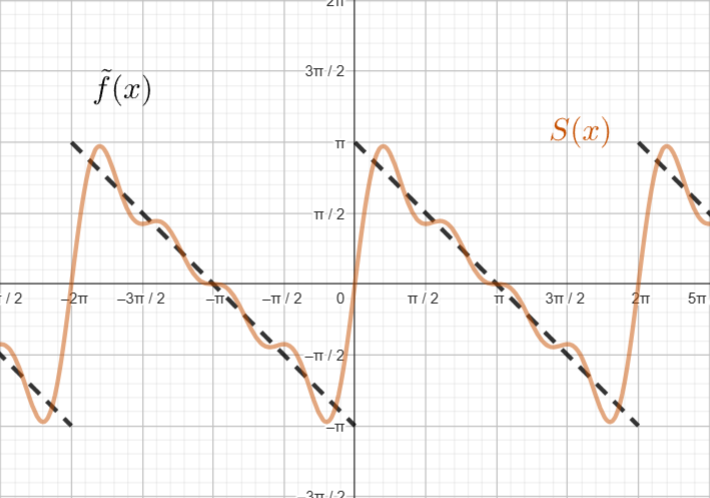
\includegraphics[width=0.5\textwidth]{addchapters1/images/addchapters1_2024_11_15_6}
    \end{multicols}

    \mediumvspace

    Заметим, что $\tilde{f}$ на $[0, 2\pi]$ имеет одно аналитическое задание (удобно интегрировать). Изменится ли 
    ряд Фурье, если сдвинуть отрезок?

    \begin{MyTheorem}
        \Ths Сдвиг промежутка длиной $2\pi$ не меняет ряда Фурье
    \end{MyTheorem}

    \begin{MyTheorem}
        \Ths Для $f : [a, b] \to \Real$ растяжение промежутка приводит к разложению:

        $b - a = 2l = T$ - период

        $a_0 = \frac{1}{l} \int_{-l}^l f(x) dx$

        $a_n = \frac{1}{l} \int_{-l}^l f(x) \cos \frac{\pi n}{l} x dx$

        $b_n = \frac{1}{l} \int_{-l}^l f(x) \sin \frac{\pi n}{l} x dx$
    \end{MyTheorem}
% end addchapters1_2024_11_15.tex

% begin addchapters1_exam_list.tex
\section{X. Программа экзамена в 2024/2025}

\begin{center}
    \textbf{1. Числовые ряды.}
\end{center}

\begin{enumerate}
    \item Определение числового ряда, понятие суммы ряда.
    \item Сходимость числового ряда. Эталонные ряды: геометрический, гармонический.
    \item Условия сходимости рядов: необходимое условие, критерий Коши.
    \item Знакоположительные числовые ряды, свойства.
    \item Признаки сходимости знакоположительных числовых рядов: признаки сравнения.
    \item Признак Даламбера, радикальный признак Коши.
    \item Интегральный признак сходимости.
    \item Знакочередующиеся ряды. Теорема Лейбница. Оценка остатка ряда.
    \item Знакопеременные ряды. Абсолютная и условная сходимость.

\begin{center}
    \textbf{2. Функциональные ряды.}
\end{center}

    \item Функциональные ряды. Сходимость. Поточечная и равномерная сходимость ряда.
    Мажорирующий ряд.
    \item Признак Вейерштрасса.
    \item Непрерывность суммы ряда.
    \item Свойства равномерно сходящихся рядов (дифференцирование и интегрирование суммы
    ряда).
    \item Степенные ряды. Теорема Абеля. Радиус сходимости.
    \item Ряд Тейлора. Стандартные разложения элементарных функций.
    \item Ортогональные системы функций и ряды Фурье. Определение тригонометрического ряда
    Фурье для функции на отрезке $[-\pi, \pi]$. Теорема Дирихле.
    \item Тригонометрический ряд Фурье на произвольном отрезке (сдвиг, растяжение)
\end{enumerate}
% end addchapters1_exam_list.tex



\end{document}

